\documentclass[../main.tex]{subfiles}

\begin{document}
\section{Numerical framework}\label{sec:theory}

This work investigates the amplification of Tollmien--Schlichting (TS) waves in a two-dimensional, incompressible flow. The governing equations are the 2D incompressible Navier--Stokes equations, defined on a domain $\Omega \subset \mathbb{R}^2$. In dimensionaless form, the equations read
\begin{equation}
	\begin{aligned}
		\partial_t \vf{u} + (\vf{u} \cdot \vf\nabla) \vf{u} & = -\vf\nabla p + \nu \Delta \vf{u} \\
		\vf\nabla \cdot \vf{u}                              & = 0,
	\end{aligned}
	\label{eq:nsdimless}
\end{equation}
where $\mathbf{u} = (u, v)$ denotes the velocity field, with $u$ and $v$ representing the horizontal and vertical velocity components, respectively; $p$ is the pressure, and $\nu$ is the kinematic viscosity. These equations are supplemented by appropriate initial and boundary conditions. The system is non-dimensionalized by selecting the boundary-layer displacement thickness $\delta^*$ as the characteristic length scale. Specifically, we set $\delta^*_{ue} = 1$ at the upstream edge of the gap in a smooth surface without discontinuities. The reference velocity is taken as the free-stream velocity $u_\infty$ at the top boundary. The corresponding Reynolds number based on $\delta^*$ is defined as
\[
	\Rey_{\delta^*} := \frac{u_\infty \delta^*_{ue}}{\nu} = \frac{1}{\nu}.
\]


\subsection{Numerical implementation}\label{sec:numericalimplementation}

To solve the dimensionless equations~\eqref{eq:nsdimless}, we employ a velocity-correction scheme implemented within a spectral-$hp$ element framework, provided by the open-source library \texttt{Nektar++}~\cite{nektaruserguide}.

Temporal discretization is performed using a second-order implicit-explicit (IMEX) splitting scheme~\cite{velocitycorrectionscheme}, resulting in the semi-discrete form
\begin{equation}
	\partial_t\vf{u}^{n+1}+ \vf{N}(\vf{u}^{n+1}) = - \grad p^{n+1} + \nu \laplacian \vf{u}^{n+1},
	\label{eq:nsdiscretized}
\end{equation}
where $\vf{N}(\vf{u}^{n+1}) := (\vf{u}^{n+1} \cdot \grad) \vf{u}^{n+1}$ is the nonlinear advection term. The time derivative is approximated using a second-order backward differentiation formula:
\begin{equation}
	\partial_t{\vf{u}^{n+1}}= \frac{\alpha \vf{u}^{n+1} - \vf{\widehat{u}}^n}{\Delta t}.
	\label{eq:timederivative}
\end{equation}
Here $\alpha = 3/2$ and $\vf{\widehat{u}}^n := 2\vf{u}^n - \frac{1}{2}\vf{u}^{n-1}$. The nonlinear advection term is extrapolated as
\begin{equation}
	\vf{N}^{n+1} = \vf{N}^{*,n+1} + \mathcal{O}(\Delta t^2), \quad \text{where } \vf{N}^{*,n+1} := 2\vf{N}^n - \vf{N}^{n-1}
	\label{eq:nonlinearextrapolation}
\end{equation}
to maintain second-order accuracy.

The velocity correction scheme proceeds in four stages:
\begin{enumerate}
	\item Compute a temporary velocity field $\vf{\tilde{u}}^{n+1}$ which includes the nonlinear advection term:
	      \begin{equation}
		      \frac{\vf{\tilde{u}}^{n+1} - \vf{\widehat{u}}^n}{\Delta t} = -\vf{N}^{*,n+1}.
		      \label{eq:tempvelocity}
	      \end{equation}
	\item Solve a Poisson equation for the pressure:
	      \begin{equation}
		      \Delta p^{n+1} = \frac{1}{\Delta t} \divp \vf{\tilde{u}}^{n+1}.
		      \label{eq:poissonpressure}
	      \end{equation}
	\item Project the velocity onto a divergence-free space:
	      \begin{equation}
		      \frac{\vf{\bar{u}}^{n+1} - \vf{\tilde{u}}^{n+1}}{\Delta t} = - \grad p^{n+1}, \quad \divp \vf{\bar{u}}^{n+1} = 0.
		      \label{eq:tempvelocitypressure}
	      \end{equation}
	\item Solve the Helmholtz equation for the updated velocity:
	      \begin{equation}
		      \frac{\alpha\vf{u}^{n+1} - \vf{\bar{u}}^{n+1}}{\Delta t} = \nu \laplacian \vf{u}^{n+1} \implies
		      \laplacian \vf{u}^{n+1} - \frac{\alpha}{\nu \Delta t} \vf{u}^{n+1} = - \frac{1}{\nu \Delta t} \vf{\bar{u}}^{n+1} .
					\label{eq:helmholtzvelocity}
	      \end{equation}
\end{enumerate}

The corresponding boundary conditions are detailed in~\cref{sec:boundaryconditions}. A schematic of the full time-integration loop is shown in~\cref{fig:vcs2d}.

\begin{figure}[ht]
	\centering
	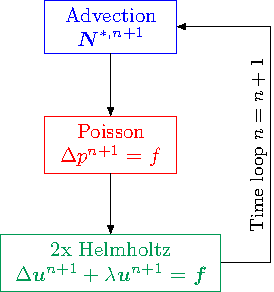
\includegraphics[width=0.35\textwidth]{../../Images/vcs2d.pdf}
	\caption{Schematic of each time step in the velocity correction scheme. Image extracted from \cite{nektaruserguide}.}
	\label{fig:vcs2d}
\end{figure}

Spatial discretization is carried out using a spectral-$hp$ element method with a continuous Galerkin formulation. The discrete space of admissible velocity fields is defined as
\begin{equation}
	\{\vf{u} \in H^1(\Omega)\times H^1(\Omega): \vf{u} \in \mathcal{P}_p(\Omega)\times \mathcal{P}_p(\Omega)\},
\end{equation}
where $\mathcal{P}_p(\Omega)$ denotes the space of polynomials in $\Omega$ of degree at most $p$. A basis polynomials of this space are defined in the square $[-1,1]^2$ and each basis function is formed as a tensor product $\phi_{ij}(x,y) = \phi_i(x)\phi_j(y)$ with $\phi_i$ being the $i$-th Legendre polynomial defined in $[-1,1]$~\cite{spectralhpSpencerBible}. For the sake of clarity, we will denote the basis functions simply as $\phi_{i}$, with the index $i$ ranging from 0 to $p^2-1$.

The weak form of~\eqref{eq:poissonpressure} is obtained by testing with $\phi_{i}$ and using the divergence theorem:
\begin{equation}
	 -\int_\Omega \grad \phi_{i} \cdot \grad p^{n+1} +\int_{\partial\Omega} \phi_{i} \grad p^{n+1} \cdot \vf{n} = \frac{1}{\Delta t} \int_\Omega \phi_{i} \divp \vf{\tilde{u}}^n.
	 \label{eq:weakpoissonpressure}
\end{equation}
Similarly, the weak form of the Helmholtz equation~\eqref{eq:helmholtzvelocity} reads
\begin{equation}
	-\int_\Omega \grad \phi_{i} \cdot \grad \vf{u}^{n+1} + \int_{\partial\Omega} \phi_{i} \grad \vf{u}^{n+1} \cdot \vf{n} - \frac{\alpha}{\nu \Delta t} \int_\Omega \phi_{i} \vf{u}^{n+1} = -\frac{1}{\nu \Delta t} \int_\Omega \phi_{i} \vf{\bar{u}}^{n+1}.
	\label{eq:weakhelmholtzvelocity}
\end{equation}
These weak formulations result in linear systems whose solution is discussed in~\cref{sec:solving}.

\subsection{Domain and boundary conditions}\label{sec:boundaryconditions}

Following the approach of~\cite{ganlinThesis}, we consider a rectangular computational domain with a sharp rectangular cavity (referred to as a gap) located on the bottom wall (see~\cref{fig:gapdomain}). The gap is fully characterized by its width $w$ and depth $d$.

\begin{figure}[ht]
	\centering
	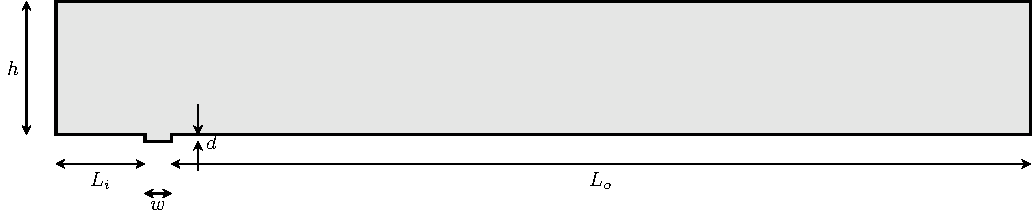
\includegraphics[width=0.65\textwidth]{../../Images/domain.pdf}
	\caption{Computational domain. The dimensions have been heterogeneously rescaled to enhance visualization of the gap geometry.}
	\label{fig:gapdomain}
\end{figure}

The dimensions defining the domain are set as $h = 150\dstar$, $\ell_\text{i} = 100\dstar$, $\ell_\text{o} = 1000\dstar$, with gap parameters $w/\dstar \in [0,130]$ and $d/\dstar \in [0,4]$. These values are chosen to ensure that all relevant physical phenomena are captured while keeping computational costs manageable.

The domain is discretized using $N_\text{e}$ non-overlapping elements. The value $N_\text{e}$ varies depending on the dimensions of the gap, but it is typically of the order of 10\,000. Elements near the boundary layer are quadrilateral, while those farther from the wall, particularly near the top of the domain, are triangular. A schematic of the mesh is shown in~\cref{fig:mesh}. To satisfy the requirements of the continuous Galerkin method, a conforming mesh is used.

Quadrilateral elements are preferred in the boundary layer region due to their ability to support exact integration and differentiation operations, unlike triangular elements~\cite{spectralhpSpencerBible}. Triangular elements are placed outside the boundary layer region to allow for rapid expansion in element size. To mitigate the influence of the Courant--Friedrichs--Lewy (CFL) condition near the edges of the gap, the outer quadrilateral layer is locally reduced in extent, and the remaining region is discretized using triangular elements. This hybrid meshing strategy preserves high spatial resolution while permitting a larger time step in the numerical simulation.

\begin{figure}[ht]
	\centering
	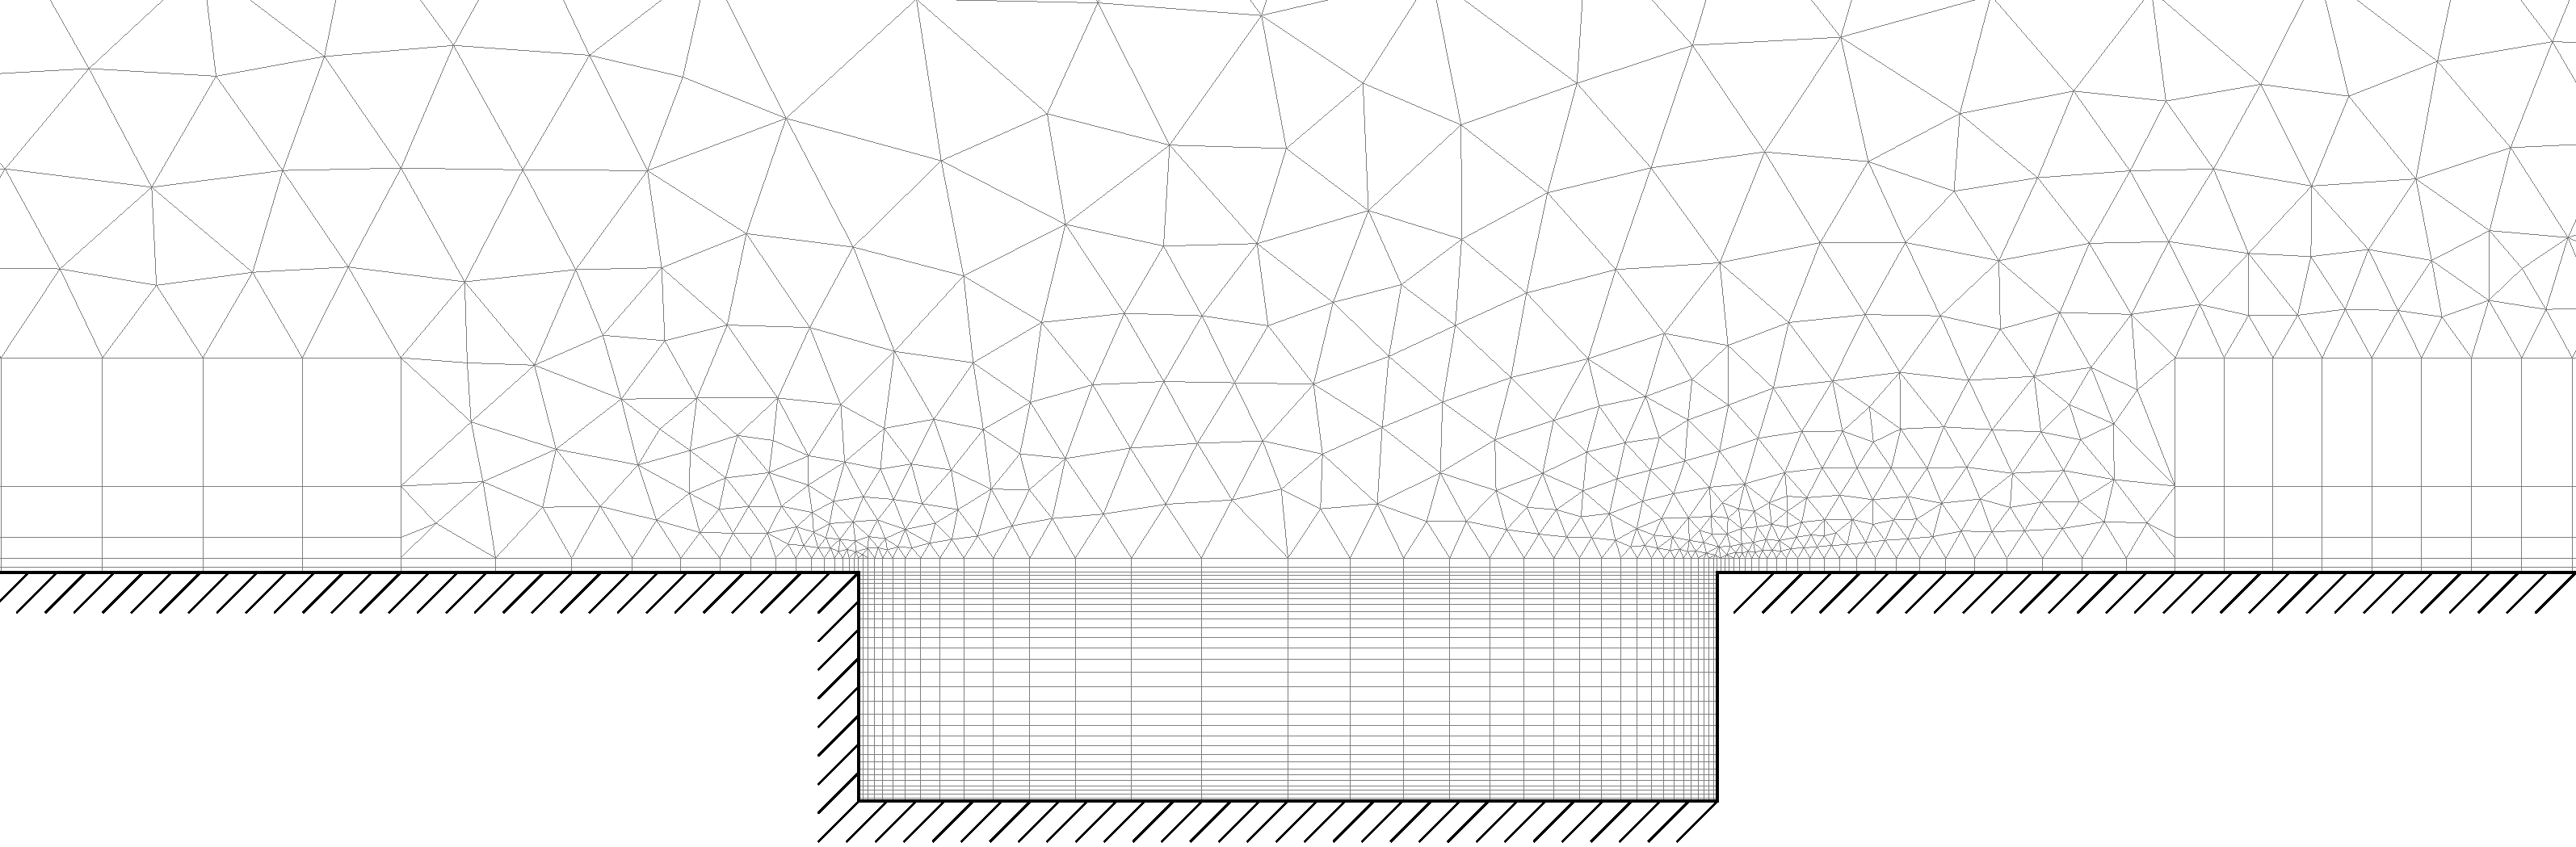
\includegraphics[width=\textwidth]{../../Images/mesh.pdf}
	\caption{Zoomed-in, unscaled view of the mesh near the gap. The configuration shown corresponds to a gap with dimensions $w = 15\dstar$ and $d = 4\dstar$. The mesh is composed of quadrilateral elements near the boundary layer and triangular elements in the upper region. It is conforming and refined near the sharp corners of the gap.}
	\label{fig:mesh}
\end{figure}
The polynomial order is set to $p=6$ for the velocity and $p=5$ for the pressure. This choice, assigning one polynomial degree higher to the velocity field, ensures satisfaction of the inf-sup (Ladyzhenskaya--Babuška--Brezzi) condition~\cite{infsupCondition,nektar}, which guarantees the existence and uniqueness of solutions to the Stokes problem.

Boundary conditions are imposed on all four sides of the domain: inflow (left), outflow (right), top, and bottom.

At the inflow, a fully developed Blasius boundary layer profile is prescribed. The Blasius profile is a self-similar solution of the boundary layer equations for incompressible, 2D, flat-plate flow with zero pressure gradient, i.e., $\partial_x p = 0$. The governing boundary layer equations in this case are
\begin{equation}
	\begin{aligned}
		u \partial_x u + v \partial_y u & = \nu \partial_{yy} u \\
		\partial_x u + \partial_y v                    & = 0.
	\end{aligned}
	\label{eq:boundarylayer}
\end{equation}
Blasius showed that these equations admit a self-similar solution through the substitution~\cite{blasius1908grenzschichten}
\begin{equation}
	\begin{aligned}
		\eta    & = y \sqrt{\frac{u_\infty}{\nu x}}    \\
		f(\eta) & = \frac{\psi}{\sqrt{\nu u_\infty x}},
	\end{aligned}
	\label{eq:blasius}
\end{equation}
where $\psi$ is the streamfunction defined by $u = \partial_y \psi$, $v = -\partial_x \psi$. From this formulation, the velocity components become
\begin{equation}
	\begin{aligned}
		u & = u_\infty f'(\eta),                                                    \\
		v & = \frac{1}{2} \frac{u_\infty}{\sqrt{\Rey_x}} (\eta f'(\eta) - f(\eta)),
	\end{aligned}
	\label{eq:blasiusuv}
\end{equation}
where $\Rey_x := u_\infty x / \nu$ is the Reynolds number based on the distance from the leading edge of the plate.

Substituting~\eqref{eq:blasiusuv} into the $x$-momentum equation in~\eqref{eq:boundarylayer} yields the classical Blasius equation,
\begin{equation}
	f''' + \frac{1}{2} f f'' = 0.
	\label{eq:blasiusODE}
\end{equation}
The equation is defined in $\eta \in[0,\infty)$ and it is equipped with boundary conditions derived from~\eqref{eq:blasiusuv}: $f(0) = 0$, $f'(0) = 0$, and $\lim_{\eta\to\infty} f'(\eta) = 1$.

This third-order ODE is solved using \texttt{solve\_bvp} from the \texttt{scipy} Python library~\cite{scipy}, which implements a fourth-order collocation method solved iteratively using Newton’s method. As the resulting velocity profile cannot be directly imported into \texttt{Nektar++}, we fit it using rational functions of degree 11, ensuring that the relative error in the $\mathcal{C}^1$ norm
\begin{equation}
	\norm{f}_{\mathcal{C}^1} := \norm{f}_\infty + \norm{f'}_\infty
\end{equation}
remains below $10^{-5}$. The resulting fit reads 
\begin{equation}
	\tilde{u}_\text{BL}(\eta) =
	\begin{cases}
		\dfrac{p(\eta)}{q(\eta)} & \text{if } \eta < \eta_\text{max},    \\
		u_\infty                 & \text{if } \eta \geq \eta_\text{max},
	\end{cases}
\end{equation}
where $p, q \in \mathcal{P}_{11}(\mathbb{R})$ and $\eta_\text{max} = 12$ is the cutoff point for the fit. A similar fit is constructed for the wall-normal velocity component. The resulting relative errors are
\begin{equation}
	\frac{\norm{\tilde{u}_\text{BL}(\eta) - u}_{\mathcal{C}^1}}{\norm{u}_{\mathcal{C}^1}} < 10^{-5}, \quad
	\frac{\norm{\tilde{v}_\text{BL}(\eta) - v}_{\mathcal{C}^1}}{\norm{v}_{\mathcal{C}^1}} < 10^{-5}.
	\label{eq:blasiusfit}
\end{equation}
To impose a consistent pressure boundary condition at the inflow that preserves the time accuracy~\cite{nektardeveloperguide}, we take the dot product of~\eqref{eq:nsdiscretized} with the normal vector $\vf{n}$ to obtain
\begin{equation}
	\partial_{\vf{n}} p^{n+1} = \left( \nu \laplacian \vf{u}^{n+1} - \partial_t \vf{u}^{n+1} - \vf{N}(\vf{u})^{n+1} \right) \cdot \vf{n}.
	\label{eq:blasiuspressurepre}
\end{equation}
Using the vector identity $\laplacian \vf{u} = \grad(\divp \vf{u}) + \rotp \rotp \vf{u}$ and enforcing incompressibility (up to the time accuracy set, in this case $\mathcal{O}(\Delta t^2)$), we arrive at a high-order Neumann boundary condition,
\begin{equation}
	\partial_{\vf{n}} p^{n+1} = \left( \nu \rotp \rotp \vf{u}^{*,n+1} - \partial_t \vf{u}^{*,n+1} - \vf{N}(\vf{u})^{*,n+1} \right) \cdot \vf{n}.
	\label{eq:pressureBC}
\end{equation}
At the outflow, the simplest choice is to impose fully developed flow conditions, i.e., $\partial_{\vf{n}} \vf{u} = 0$ and $p = 0$. However, this can become unstable in the presence of energetic vortices~\cite{nektaruserguide,outflowBoundaryCondition}. An alternative, more stable pressure Dirichlet condition is proposed in~\cite{outflowBoundaryCondition} as
\begin{equation}
	p^{n+1} = \nu \vf{n} \cdot \vf\nabla \vf{u}^{*,n+1} \cdot \vf{n} - \frac{1}{2} \norm{\vf{u}^{*,n+1}}^2 S(\vf{n}\cdot \vf{u}^{*,n+1}),
	\label{eq:outflowBC}
\end{equation}
where $S(\vf{n} \cdot \vf{u}) = \frac{1}{2}(1 - \tanh(\vf{n} \cdot \vf{u} / (\vf{u}_0 \varepsilon)))$ is a smooth step function, $\vf{u}_0$ is a reference velocity, and $\varepsilon$ controls the steepness of the step.

Once $p^{n+1}$ is known, the velocity at the boundary is set via
\begin{equation}
	\vf{u}^{n+1} = \frac{1}{\nu} \left[ p^{n+1} \vf{n} + \frac{1}{2} \norm{\vf{u}^{*,n+1}}^2 S(\vf{n} \cdot \vf{u}^{*,n+1}) \vf{n} - \nu \grad \vf{u}^{*,n+1} \cdot \vf{n} \right].
	\label{eq:outflowBCu}
\end{equation}
At the top boundary, we impose free-stream conditions: $u = u_\infty$, $v = v_\infty(x)$, and the pressure condition from~\eqref{eq:pressureBC}. We stress that the wall-normal velocity is $x$-dependent, as inherited from the Blasius profile. On the bottom wall, a no-slip condition is applied: $u = 0$, $v = 0$, and the pressure condition again follows~\eqref{eq:pressureBC}, which reduces to the standard Neumann condition $\partial_{\vf{n}} p^{n+1} = 0$ in this case.

\subsection{Solving the linear systems}\label{sec:solving}

In this section, we briefly outline the procedure used to solve the weak form of the pressure Poisson equation~\eqref{eq:weakpoissonpressure}. The same approach applies analogously to the weak form of the velocity Helmholtz equation~\eqref{eq:weakhelmholtzvelocity}.

Integration is performed on an element-by-element basis. Let $\Omega_e \subset \Omega$ denote a single element. Using~\eqref{eq:weakpoissonpressure} together with the boundary condition from~\eqref{eq:pressureBC}, the elementwise pressure equation becomes
\begin{equation}
	\int_{\Omega_e} \grad \phi_{i} \cdot \grad p_e^{n+1} = -\frac{1}{\Delta t} \int_{\Omega_e} \phi_{i} \divp \vf{\tilde{u}}_e^n + \int_{\partial\Omega_e} \phi_{i} \left( \nu \rotp \rotp \vf{u}_e^{*,n+1} - \partial_t \vf{u}_e^{*,n+1} - \vf{N}(\vf{u}_e)^{*,n+1} \right) \cdot \vf{n},
	\label{eq:weakpoissonpressureelement}
\end{equation}
where the subscript $e$ indicates that the quantities are relative to the element $\Omega_e$. 

Assume that each physical element is obtained from a reference element via a mapping $\Omega_e = \boldsymbol{\varphi}_e(\Omega_{\mathrm{st}})$, where $\Omega_{\mathrm{st}}$ refers to either the standard square element
\begin{equation}
	\mathcal{Q}_\text{st} := \{ (\eta_1, \eta_2) \in \mathbb{R}^2 : -1 \leq \eta_1, \eta_2 \leq 1 \}
\end{equation}
or the standard triangular element
\begin{equation}
	\mathcal{T}_\text{st} := \{ (\xi_1, \xi_2) \in \mathbb{R}^2 : -1 \leq \xi_1 \leq 1, \ -1 \leq \xi_2 \leq 1, \ \xi_1 + \xi_2 \leq 0 \}.
\end{equation}
It is noted that to construct tensor-product basis functions $\phi_i$ on $\mathcal{T}_\text{st}$, a collapsing-coordinates mapping is employed. One such mapping is given by
\begin{equation}
\xi_1 = \frac{(1+\eta_1)(1-\eta_2)}{2} - 1, 
\quad
\xi_2 = \eta_2,
\label{eq:collapsingmapping}
\end{equation}
which maps the square $\mathcal{Q}_\text{st}$ to the triangle $\mathcal{T}_\text{st}$ as shown in~\cref{fig:squareTriangle}. 

\begin{figure}[ht]
  \centering
	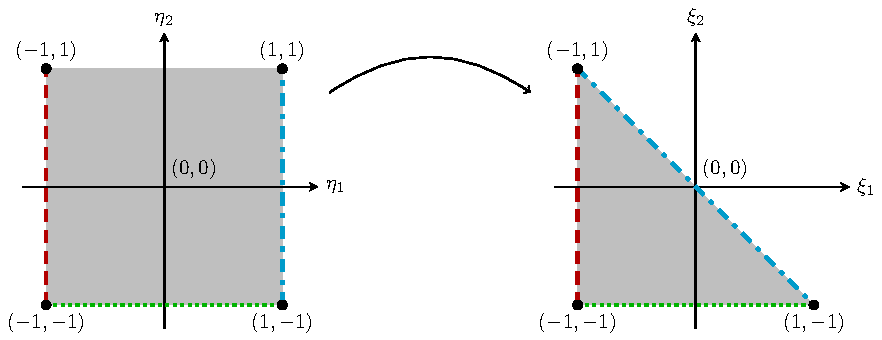
\includegraphics[width=0.8\textwidth]{../../Images/squareTriangle.pdf}
	\caption{Collapsing-coordinates mapping from the standard square element $\mathcal{Q}_\mathrm{st}$ to the standard triangular element $\mathcal{T}_\mathrm{st}$, as defined in~\eqref{eq:collapsingmapping}. The line styles on the element edges illustrate how the boundaries are transformed under the mapping.}
	\label{fig:squareTriangle}
\end{figure}

The pressure field is then expanded spectrally in terms of the basis functions as
\begin{equation}
p_e^{n+1} = \sum_{i=0}^{p^2-1} \hat{p}_{i,e}^{n+1} \, \phi_i .
\end{equation}
Substituting this expansion into~\eqref{eq:weakpoissonpressureelement} yields the following linear system for each element
\begin{equation}
	\vf{M}_e \vf{\hat{p}}_e^{n+1} = \vf{f}_e.
	\label{eq:poissonlinearsystem}
\end{equation}
Here, $\vf{M}_e = (m_{ij}^e)$ is the elementwise mass matrix, defined as
\begin{equation}
	m_{ij}^e = \int_{\Omega_\text{st}} \grad \phi_{i} \cdot \grad \phi_{j} \, J_e,
	\label{eq:massmatrix}
\end{equation}
where $J_e = \vf{D\varphi}_e$ is the Jacobian of the element mapping. In~\eqref{eq:poissonlinearsystem}, $\vf{\hat{p}}_e^{n+1} = (\hat{p}_{i,e}^{n+1})$ is the vector of unknown pressure coefficients on element $\Omega_e$, and $\vf{f}_e = (f_{i,e}^{n+1})$ is the corresponding right-hand side vector, assumed precomputed for brevity.

The entries $m_{ij}^e$ are evaluated using Gauss quadrature with a sufficient number of points to ensure exact integration on quadrilateral elements. For more details on quadrature choices and integration accuracy, see~\cite{spectralhpSpencerBible}. In practice, the integral in~\eqref{eq:massmatrix} is approximated as
\begin{equation}
	m_{ij}^e = \sum_{k=1}^{N_q} w_k \, \grad \phi_{i}(\vf{x}_k) \cdot \grad \phi_{j}(\vf{x}_k) \, J_e(\vf{x}_k)
	\label{eq:massmatrixgauss}
\end{equation}
where $\vf{x}_k$ are the quadrature points and $w_k$ are the associated weights, typically the product of 1D Gauss–Legendre weights for tensor-product elements.

Due to the continuous Galerkin formulation, certain degrees of freedom (DoFs) are shared between adjacent elements. To define the global system, let
\begin{equation}
	p_\text{gl}^{n+1} = \sum_{i=0}^{N_\text{dof}-1} \hat{p}_{i,\text{gl}}^{n+1} \phi_i,
\end{equation}
and introduce the global coefficient vector $\vf{\hat{p}}_\text{gl}^{n+1} = (\hat{p}_{i,\text{gl}}^{n+1})$, and the local coefficient vector $\vf{\hat{p}}_{\text{loc}}^{n+1} = (\vf{\hat{p}}_{i,e}^{n+1})_{\substack{0 \leq i < p^2\\0 \leq e < N_\text{e}}}$. Then, the global and local vectors are related via an assembly operator
\begin{equation}
	\vf{\hat{p}}_\text{loc}^{n+1} = \vf{\mathcal{A}} \vf{\hat{p}}_{\text{gl}}^{n+1},
	\label{eq:globalpressure}
\end{equation}
where $\bm{\mathcal{A}}$ is a sparse Boolean matrix (consisting of zeros and ones) that encodes the connectivity between local and global DoFs. Using this relation, we construct the global mass matrix $\vf{M}_\text{gl}$, which is assembled from the local elemental mass matrices. These local contributions are combined according to the assembly matrix, resulting in shared entries that reflect the continuity of degrees of freedom across element boundaries. For detailed information on the implementation and mathematical formulation of the spectral-$hp$ element method, refer to~\cite{spectralhpSpencerBible}. This leads to a linear system of the form
\begin{equation}
\vf{M}_\text{gl} \vf{\hat{p}}_\text{gl}^{n+1} = \vf{\hat{f}}_\text{gl}^{n+1},
\end{equation}
which must be solved at each time step.


\section{Linear stability analysis}\label{sec:lst}

We initiate the nonlinear simulations using a smooth initial condition. Depending on the gap geometry, the flow may evolve towards a steady state or display sustained oscillatory behavior. In cases where the solution converges to a steady flow, denoted by $\vf{U}(x, y)$, this state can be used as a critical point to perform a linear stability analysis around it.

To study the evolution of small-amplitude perturbations, we decompose the velocity field as
\begin{equation}
    \vf{u}(x, y, t) = \vf{U}(x, y) + \vf{u}'(x, y, t),
\end{equation}
where $\vf{u}'=(u',v')$ denotes the perturbation field, and $u'$ and $v'$ are the perturbation components in the streamwise and wall-normal directions, respectively. Substituting this decomposition into the full Navier--Stokes equations and retaining only terms linear in $\vf{u}'$, we obtain the linearized Navier--Stokes equations:
\begin{equation}
	\begin{aligned}
		\partial_t \vf{u}' + (\vf{U} \cdot \grad) \vf{u}' + (\vf{u}' \cdot \grad) \vf{U} & = -\grad p' + \nu \Delta \vf{u}' \\
		\grad \cdot \vf{u}'                                                              & = 0.
	\end{aligned}
	\label{eq:linearizedns}
\end{equation}
Unless otherwise stated, we hereafter omit the prime notation and denote the perturbation field simply as $\vf{u}$. 
% The system~\eqref{eq:linearizedns} can be expressed in operator form as an initial value problem:
% \begin{equation}
% 	\partial_t \vf{u} = \vf{\mathcal{L}} \vf{u},
% 	\label{eq:linearizednsoperator}
% \end{equation}
% where the linearized Navier--Stokes operator $\vf{\mathcal{L}}$ is defined by
% \begin{equation}
%     \vf{\mathcal{L}}\vf{u} := -(\vf{U} \cdot \grad) \vf{u} - (\vf{u} \cdot \grad) \vf{U} + \nu \Delta \vf{u} - \grad p.
% \end{equation}
% The incompressibility constraint $\grad \cdot \vf{u} = 0$ must also be enforced.

% This formulation enables the analysis of the stability properties of the baseflow $\vf{U}(x,y)$ by examining the spectrum of the linear operator $\vf{\mathcal{L}}$ and the time evolution of perturbations governed by~\eqref{eq:linearizednsoperator}.
% \subsection{Local stability theory}

% Local stability theory (LST) relies on the assumption that the baseflow $\vf{U}(x,y)$ is parallel, i.e., it does not vary in the streamwise direction $x$. Under this assumption, and using the incompressibility condition and boundary constraints, the baseflow must take the form $\vf{U}(y) = (U(y), 0)$. Imposing this structure, the linearized Navier--Stokes equations~\eqref{eq:linearizedns} simplify to~\cite{schmid2001stability}:
% \begin{equation}
% 	\begin{aligned}
% 		\partial_t u + U \partial_x u + v \partial_y U & = -\partial_x p + \nu \Delta u \\
% 		\partial_t v + U \partial_x v                  & = -\partial_y p + \nu \Delta v \\
% 	\end{aligned}
% 	\label{eq:linearizednsparallel}
% \end{equation}
% with the pressure satisfying the associated Poisson equation:
% \begin{equation}
% 	\laplacian p = -2 \partial_y U \partial_x v
% 	\label{eq:poissonpressureparallel}
% \end{equation}
% Substituting~\eqref{eq:poissonpressureparallel} into~\eqref{eq:linearizednsparallel} and eliminating pressure, the wall-normal velocity component $v$ satisfies a fourth-order partial differential equation:
% \begin{equation}
% 	\left[(\partial_t + U \partial_x)\laplacian - \partial_{y}^2 U \partial_x  + \laplacian^2\right]v = 0
% \end{equation}
% This equation is subject to boundary conditions at the wall $y = 0$ ($v = \partial_y v = 0$) and in the free-stream limit $y \to \infty$ ($v, \partial_y v \to 0$). Once $v$ is computed, the streamwise velocity component $u$ can be recovered from the continuity equation.

% We now apply a Fourier transform in the streamwise direction $x$ and a Laplace transform in time $t$, yielding the classical Orr-Sommerfeld equation~\cite{schmid2001stability}:
% \begin{equation}
% 	\left[(-\ii\omega + \ii\alpha U) (\partial_y^2 - \alpha^2) - \ii\alpha \partial_y^2 U - \nu (\partial_y^2 - \alpha^2)^2\right] \tilde{v} = 0
% \end{equation}
% Here, $\alpha$ denotes the streamwise wavenumber, $\omega$ is the frequency of the perturbation, and $\tilde{v}$ is the Fourier-transformed wall-normal velocity. The physical form of $v$ is then reconstructed as:
% \begin{equation}
% v(x,y,t) = \sum_{\alpha,\omega} \tilde{v}_{\alpha,\omega}(y) \exp{\ii\alpha x - \ii\omega t}
% 	\label{eq:fourierlaplacetransform}
% \end{equation}
% where the sum is taken over the discrete spectrum of the Orr-Sommerfeld operator.

% Several solution approaches exist in the literature~\cite{schmid2001stability}. In this work, we adopt a \emph{spatial stability analysis}, in which we fix $\omega \in \mathbb{R}$ and solve for complex-valued $\alpha = \alpha_\text{r} + \ii \alpha_\text{i} \in \mathbb{C}$. In this formulation, $\omega$ corresponds to the physical (real-valued) frequency of the perturbation, $\alpha_\text{r}$ represents the spatial wavenumber, and $\alpha_\text{i}$ is the spatial growth rate.

\subsection{\texorpdfstring{$e^N$}{eN}-method}

The $e^N$ method is a widely used approach in linear stability theory to quantify the amplification of disturbances in a flow. Its main assumption is that a perturbation of amplitude (yet to be defined) $A(x_0)$ at a reference position $x_0$ evolves in the streamwise direction $x$ according to
\begin{equation}
	A(x) = A(x_0) \exp{n_{x_0}(x)},
	\label{eq:amplitudeEvolution}
\end{equation}
where $n_{x_0}(x)$ denotes the $n$-factor, which can be recovered from
\begin{equation}
	n_{x_0}(x) = \log\left( \frac{A(x)}{A(x_0)} \right).
	\label{eq:nfactorAmplitude}
\end{equation}
Henceforth, we omit the subscript $x_0$ for simplicity. A suitable definition for the amplitude in the wall-normal direction remains to be specified. In our setup, we choose the $L^\infty$ norm of the velocity magnitude $\vf{u}$,
\begin{equation}
	A(x) := \norm{\vf{u}(x,y)}_{L^\infty(\mathcal{Y}(x))} = \max_{y \in \mathcal{Y}(x)} |\vf{u}(x,y)| = \max_{y \in \mathcal{Y}(x)} \sqrt{u(x,y)^2 + v(x,y)^2},
	\label{eq:amplitudeNorm}
\end{equation}
where $\mathcal{Y}(x)$ denotes the wall-normal domain at a given streamwise position $x$. Since the perturbation vanishes at the boundaries and the solution remains bounded, the maximum value is guaranteed to be attained within the domain.


% Within the framework of spatial local stability theory, once an appropriate amplitude norm is defined in the wall-normal direction (such as the $L^\infty$ or $L^2$ norm), the $n$-factor can be directly related to the spatial growth rate $\alpha_\text{i}(\omega)$ by the following integral expression:
% \begin{equation}
% 	n(x,\omega) = -\int_{x_0}^x \alpha_\text{i}(\omega) \, \dd{s}
% \end{equation}
% To characterize the maximum amplification across all frequencies, we define the $N$-factor as:
% \begin{equation}
% 	N(x) = \sup_{\omega \in \mathbb{R}} n(x,\omega)
% \end{equation}
% The $N$-factor thus quantifies the logarithmic amplification of the perturbation between $x_0$ and $x$. This scalar quantity is commonly used in transition prediction to estimate whether the flow will become unstable and whether laminar-turbulent transition may occur.
\end{document}
